% Created 2023-04-04 mar 11:11
% Intended LaTeX compiler: pdflatex
\documentclass{latex/classes/thesis}
\usepackage[utf8]{inputenc}
\usepackage[T1]{fontenc}
\usepackage{graphicx}
\usepackage{longtable}
\usepackage{wrapfig}
\usepackage{rotating}
\usepackage[normalem]{ulem}
\usepackage{amsmath}
\usepackage{amssymb}
\usepackage{capt-of}
\usepackage{hyperref}
\author{Miguel Angel Piña Avelino}
\date{\today}
\title{A Study Of Concurrent Data Structures With Relaxed Semantics}
\hypersetup{
 pdfauthor={Miguel Angel Piña Avelino},
 pdftitle={A Study Of Concurrent Data Structures With Relaxed Semantics},
 pdfkeywords={},
 pdfsubject={},
 pdfcreator={Emacs 28.2 (Org mode 9.5.5)},
 pdflang={Spanish}}
\begin{document}

\maketitle
\tableofcontents


\chapter{{\bfseries\sffamily TODO} Introduction}
\label{sec:orgcb5adb0}

\section{{\bfseries\sffamily TODO} Overview}
\label{sec:orge30a896}

\section{{\bfseries\sffamily TODO} Motivation}
\label{sec:orge43aec8}

\section{{\bfseries\sffamily TODO} Objectives and contributions}
\label{sec:org5d03641}

\section{{\bfseries\sffamily TODO} Organization}
\label{sec:org9e66e91}


\chapter{{\bfseries\sffamily TODO} Concurrent Computing}
\label{sec:orgf4db7e0}

What is concurrent computing? This is a good question. We should first talk
about single-core and multi-core processors manufactured by the computer
industry. After the second world war and until the 90's the general purpose
cpus were single-core. All processes were executed in a single-core, and the
operating systems simulated concurrency using schedulers and other
techniques. In 2001, IBM introduce the first multi-core processor
\cite{ibmIBM100Power}, it allows that two processors work together at a very
high bandwidth (for the epoch) with large on-chip memories and with
high-speed buses. Since then, the amount of cores in each processors has been
increasing. We must consider as well the Moore's law, loosely speaking, this
law tells us that each year more and more transistors are placed into the
same space (i.e. electronic components and circuits are reduced in size), but
their speed cannot be increased without overheating. Consequently, the
industry move to ``multi-core'' architectures. In this architecture multiple
processors communicate through shared memory (RAM, hardware caches),
permitting make computing more effectively using \emph{parallelism}, where the
processors work together on a single task \cite{DBLP_books_daglib_0020056}.

\section{{\bfseries\sffamily TODO} Classic concurrent computing}
\label{sec:org8eab583}

\begin{itemize}
\item[{$\square$}] Basic Definitions
\item[{$\square$}] FLP impossibility result
\item[{$\square$}] Asynchronous Shared Memory
\item[{$\square$}] Primitive Synchronization Operations and Consensus
\end{itemize}


\section{{\bfseries\sffamily TODO} Relaxed concurrent computing}
\label{sec:org02d805d}

\begin{itemize}
\item[{$\square$}] Relaxing the problem
\item[{$\square$}] Multiplicity preliminaries
\item[{$\square$}] Another relaxations?
\end{itemize}

\section{{\bfseries\sffamily TODO} Work-stealing}
\label{sec:org42121cc}

\begin{itemize}
\item[{$\square$}] How it works the work-stealing
\item[{$\square$}] Classic algorithms
\item[{$\square$}] Idempotent algorithms
\item[{$\square$}] Work-stealing with multiplicity
\end{itemize}

\section{{\bfseries\sffamily TODO} Data-Structures}
\label{sec:org1560a9f}

\begin{itemize}
\item[{$\square$}] Queues with multiplicity
\end{itemize}


\chapter{{\bfseries\sffamily TODO} Preliminaries}
\label{sec:org0431166}

\section{{\bfseries\sffamily TODO} Mathematical model}
\label{sec:org671299f}

\section{{\bfseries\sffamily TODO} Realistic model of computation}
\label{sec:org7494683}

We consider a standard concurrent shared memory system with \(n \ge 2\)
\emph{asynchronous} processes, \(p_0, \ldots, p_{n-1}\), which may crash at any time
during an execution. The processes communicate with each other by invoking
atomic instructions of base objects: either simple Read/Write instructions to
\textbf{atomic objects}, or more powerful \textbf{Read-Modify-Write} instructions, such as
\texttt{Test-And-Set}, \texttt{Swap} or \texttt{Compare-And-Set}.

For simplicity we assume a single multicore chip where the processes run. In
our system we consider a memory hierarchy, where we have the following
elements in the hierarchy:

\begin{itemize}
\item Cache memory
\item Memory bus
\item Main memory
\end{itemize}

In this model, each processor core may read and
write to a single shared memory space. Usually each processor core has a
cache to operate with data from the shared memory. Often, this data is
transferred through a memory bus, allowing connect the processors with the
memory. The figure \ref{fig:arch} shows a simplified view of this model. In
the sections: \hyperref[sec:org4f1ae3f]{Cache memory}, \hyperref[sec:org67270de]{Memory bus} and \hyperref[sec:org3314b85]{Main memory}, we explain more in
detail the meaning of each bullet of the list.

\begin{figure}
\begin{minipage}{\linewidth}
  \includesvg[width=\linewidth]{figs/architecture}
\end{minipage}
\caption{Simplified view of a modern computer system cache architecture}
\label{fig:arch}
\end{figure}


\subsection{Cache memory}
\label{sec:org4f1ae3f}

The cache memory is a special very high-speed memory that is very close to
the processor and the processes can access it very fast. The caches are used
to reduce average latencies to access storage structures
\cite{DBLP_series_synthesis_2020Nagarajan}. In recent multicore chips, the
cache memory is divided in three levels, two private levels (L1 and L2) for
each processor and a third level (L3) that is shared by the cores. The
purpose of the first two levels is to provide fast access to data and
instructions for the processors.

Each processor use the first level of cache to get the data and instructions
to execute them, usually the access to this level of cache is very fast
respect to the access to other levels.  The second level is often more
capacious than first level and is used to store data and instructions that
are close to be executed. In the third level, this cache is shared by many
processors and is used as feeder for the L2 cache.

\subsection{Memory bus}
\label{sec:org67270de}

Is a computer bus that allows transfer data from the primary memory to the
CPU and the cache memory. It is made up of two parts: the data bus and the
address bus. The data bus is in charge of transfer information between the
primary memory and the correspondent chipset.
The address bus is used to retrieve information about the location of stored
information.


\subsection{Main memory}
\label{sec:org3314b85}

Is the responsible of hold the data that CPU need to access frequently, such
as instructions or data currently being processed. The CPU can access to
this information faster than the access to secondary memory.

\subsection{Consistency Memory Model and Cache Coherence}
\label{sec:org7c75147}

\begin{enumerate}
\item Consistency memory model
\label{sec:org5476049}

Following the simplified view of the cache architecture, we want to have a
correct shared memory. And what this means? The correctness of the shared
memory can be separated into two sub-issues: \emph{consistency} and \emph{correctness}.

The consistency (definitions) provide rules about loads and stores (memory
reads and writes) and how they act upon memory. These definitions must take
into account the behaviour of those operations on memory through access of
multiple threads or even a single thread. The consistency models define
correct shared memory behavior in terms of loads and stores, without
reference to caches or coherence \cite{DBLP_series_synthesis_2020Nagarajan}.
Shared memory correctness is specified by a memory consistency model (or
memory model). This specifies the allowed behavior of multithreaded programs
executing with shared memory.

The most intuitive and strongest memory model is the \emph{Sequential Consistency}
(SC). Another memory model used by systems \emph{x86} and \emph{SPARC} is \emph{Total Store Order}
(TSO), motivated by the desire of use \emph{first-in-first-out} write buffers to
hold the results of committed stores before writing results to the caches.
Additional to the prior memory model, "relaxed" or "weak" memory models are
considered, because these models shows that most memory orderings in strong
models are unnecessary \cite{DBLP_series_synthesis_2020Nagarajan}.

\item Cache coherence
\label{sec:org5c9c5ee}

Cache coherence protocols are used in response to solve a coherence problem
in cache. For example, a coherence problem can arise if multiple cores have
access to multiple copies of a datum, each one in a core, and at least one
them is a write access. The cache coherence protocols prevent the access to
stale data (incoherent data); this can be done using a set of rules
implemented by the distributed set of cores within a system. These
protocols use the common MOESI coherence states: modified (M), owned (O),
exclusive (E), shared (S) and invalid (I). The protocol acts like a state
machine, moving from one state to another based on the conditions of the
data and the cache memory \cite{DBLP_series_synthesis_2020Nagarajan}.
\end{enumerate}



\subsection{Memory fences}
\label{sec:orgcf455a3}

A memory fence is a barrier instruction that causes a CPU or compiler to
enforce a an ordering constraint on memory operations (loads and stores)
issued before and after the barrier instruction.

These instructions are necessary because most modern CPUs or compilers
employ performance optimizations, changing the order of the instructions on
one program, that could result in out-of-order execution. Normally these
optimizations are unnoticed in a single thread program, but can cause an
unpredictable behavior in concurrent programs.

For example, consider the following multi-thread program, with 2
threads, each one running in one core in a concurrent way:

Thread 1, core 1
\lstset{language=c++,label= ,caption= ,captionpos=b,numbers=none}
\begin{lstlisting}
while (z == 0);
print(y);
\end{lstlisting}

Thread 2, core 2
\lstset{language=c++,label= ,caption= ,captionpos=b,numbers=none}
\begin{lstlisting}
y = 30;
z = 1;
\end{lstlisting}

In this case, we might expect that the \texttt{print(y)} always print the number 30,
nevertheless, the compiler or the CPU could change the order of the
instructions for the thread 2, giving as result an execution where the value
for \texttt{y} is undefined and the instructions could be interleaved as follows:

\lstset{language=c++,label= ,caption= ,captionpos=b,numbers=none}
\begin{lstlisting}
z = 1; // Thread 2
while (z == 0); // Thread 1
print(y); // Thread 1
y = 30; // Thread 2
\end{lstlisting}

This execution is sequentially consistent, but is an out-of-order
execution producing an undefined result. With the use of memory barriers, we
can ensure that instructions don't be reordered. For example, our code could
be rewrite as follows:

Thread 1, core 1.
\lstset{language=c++,label= ,caption= ,captionpos=b,numbers=none}
\begin{lstlisting}
while (z == 0);
fence()
print(y);
\end{lstlisting}

Thread 2, core 2.
\lstset{language=c++,label= ,caption= ,captionpos=b,numbers=none}
\begin{lstlisting}
y = 30;
fence();
z = 1;
\end{lstlisting}


Languages as \texttt{Java} or \texttt{C++} provide instructions to establish synchronization
and ordering constraints between threads without an atomic operation. These
instructions have semantics well defined for

In the case of Java, we have static methods of the class VarHandle
(\texttt{java.lang.invoke.VarHandle}) that are refered as memory fence methods which
helps to provide fine-grained control of memory ordering. These statics
methods are \cite{varHandleJdk92017}:

\begin{description}
\item[{fullFence}] Ensures that loads and stores before the fence will not be
reordered with loads and stores after the fence. This method has memory
ordering effects compatible with
\texttt{atomic\_thread\_fence(memory\_order\_seq\_cst)}.
\item[{acquireFence}] Ensures that loads before the fence will not be reordered
with loads and stores after the fence. This method has memory ordering
effects compatible with \texttt{atomic\_thread\_fence(memory\_order\_acquire)}.
\item[{releaseFence}] Ensures that loads and stores before the fence will not
be reordered with stores after the fence. This method has memory ordering
effects compatible with \texttt{atomic\_thread\_fence(memory\_order\_release)}.
\item[{loadLoadFence}] Ensures that loads before the fence will not be
reordered with loads after the fence.
\item[{storeStoreFence}] Ensures that stores before the fence will not be
reordered with stores after the fence.
\end{description}

For C++, we have the function
\texttt{std::atomic\_thread\_fence}\cite{threadFenceCpp2020}, which establishes
memory synchronization ordering of non-atomic and relaxed atomic access, as
instructed by order, without an associated atomic operation. The type of
synchronization that can handle are the following:

\begin{itemize}
\item Fence-atomic synchronization
\item Atomic-fence synchronization
\item Fence-Fence Synchronization
\end{itemize}

And using a memory order\cite{memoryOrderCpp2020}, it can specifies how
memory accesses, including regular, non atomic memory accesses, are to be
ordered around an atomic operation. In total are six orders, from the
relaxed memory order to the sequential consistent memory order. They are:
\texttt{memory\_order\_relaxed}, \texttt{memory\_order\_consume}, \texttt{memory\_order\_acquire},
\texttt{memory\_order\_acq\_rel} and \texttt{memory\_order\_seq\_cst}. A note about
\texttt{atomic\_thread\_fence} functions, is that on x86 (x86\textsubscript{64}), these functions
issue no CPU instructions and only affect compile time code, with exception
for \texttt{std::atomic\_thread\_fence(std::memory\_order::seq\_cst)}, which issue the
full memory fence instruction \texttt{MFENCE}. For other archict



\section{{\bfseries\sffamily TODO} Data-Structures}
\label{sec:orga272715}

\subsection{Queues}
\label{sec:org7bb721b}

\subsection{Stacks}
\label{sec:org2a080b8}


\section{{\bfseries\sffamily TODO} Some Hardware Foundations}
\label{sec:orgd2268c9}

\subsection{Cache memory}
\label{sec:org34f4c0a}

The cache memory

\begin{enumerate}
\item Multiple caches
\label{sec:org02364b7}


\item Cache coherence protocols
\label{sec:org3b50851}



\begin{enumerate}
\item MESI
\label{sec:orgf940c04}


\item MOESI
\label{sec:orgb2f4fe3}
\end{enumerate}


\item Store Buffers
\label{sec:orgbdc3115}
\end{enumerate}


\subsection{Reordering (CPU or Compiler)}
\label{sec:org98d1b82}

\subsection{Memory Barriers}
\label{sec:orgdebd0e5}

\begin{enumerate}
\item X86 and TSO architectures
\label{sec:orgb170e58}

\item Memory Fences
\label{sec:org565fbe5}
\end{enumerate}

\subsection{Read-Modify-Write Operations}
\label{sec:orgfc71265}

\subsection{Bibliography}
\label{sec:orgfb886e2}

\begin{itemize}
\item \url{https://blog.the-pans.com/std-atomic-from-bottom-up/}
\end{itemize}

\section{{\bfseries\sffamily TODO} C++ Memory model}
\label{sec:org6ce2eef}

\subsection{Memory model basics}
\label{sec:orgd7b56ea}

\begin{enumerate}
\item Objects and memory locations
\label{sec:orgde06649}


\item Objects, memory locations, and concurrency
\label{sec:org6ac561a}


\item Modification orders
\label{sec:org8886ab4}
\end{enumerate}


\subsection{Atomic operations and types in C++}
\label{sec:org4f446af}


\begin{enumerate}
\item The standard atomic types
\label{sec:org2e813b5}

\item Operations on std::atomic\textsubscript{flag}
\label{sec:org6ed34c5}

\item Operations on std::atomic<boolean>
\label{sec:orgb925b80}

\item Operations on std::atomic<T*>: pointer arithmetic
\label{sec:orgd5ed502}

\item Operations on standard atomic integral types
\label{sec:org58d9d65}

\item The std::atomic<> primary class template
\label{sec:orge300818}

\item Free functions for atomic operations
\label{sec:orgdebadc9}
\end{enumerate}

\subsection{Synchronizing operations and enforcing ordering}
\label{sec:org7f549f4}

\begin{enumerate}
\item The synchronization relationship
\label{sec:orge70bc05}

\item The happens-before relationship
\label{sec:org2df9e23}

\item Memory ordering for atomic operations
\label{sec:orge369927}

\item Release sequences and synchronizes-with
\label{sec:org6bc0fed}

\item Fences
\label{sec:org5f7a068}

\item Ordering non-atomic operations with atomics
\label{sec:org7f972df}

\item Ordering non-atomic operations
\label{sec:orgb957b6e}
\end{enumerate}


\section{{\bfseries\sffamily TODO} Guidelines for designing data-structures for concurrency}
\label{sec:org17ae801}

\begin{itemize}
\item Ensure that no thread can see a state where the invariants of the
data-structure have been broken by the action of the another thread.

\item Take care to avoid race conditions inherent in the interface to the
data-structure by providing functions for complete operations rather than
for operations steps.

\item Pay attention to how the data-structure behaves in the presence of
exceptions to ensure that the invariants are not broken.

\item Minimize the opportunities for deadlock when using the data-structure by
restricting the scope of locks and avoiding nested locks where possible.
\end{itemize}





\chapter{{\bfseries\sffamily TODO} Work Stealing}
\label{sec:orgf88fed7}

We analyze the algorithms for work-stealing described in the article Fully
Read/Write Fence Free Work-Stealing With Multiplicity, also the algorithm
called "Idempotent FIFO Work-Stealing", this because the algorithm have a
similar semantic than the prior algorithms.

\begin{figure}
\begin{minipage}{\linewidth}
  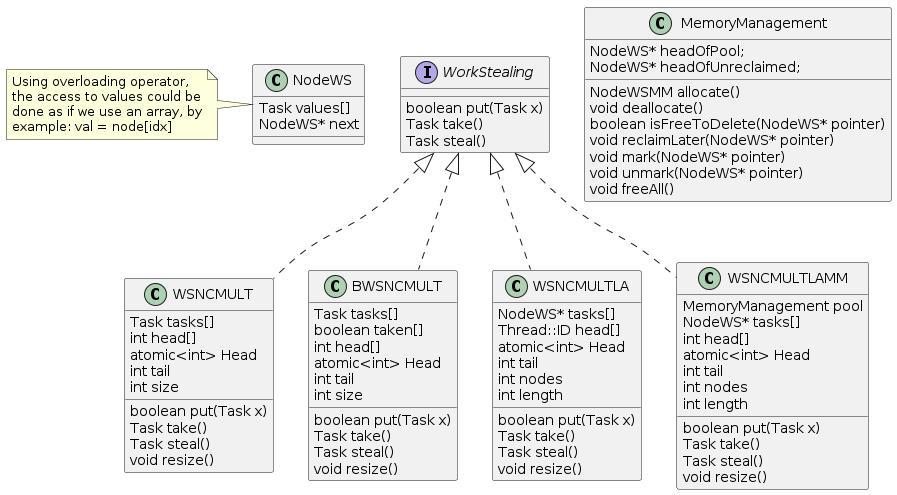
\includegraphics[width=\linewidth]{figs/objects.png}
\end{minipage}
\caption{Class Diagrama}
\label{fig:class_diagram}
\end{figure}


\section{{\bfseries\sffamily TODO} Model}
\label{sec:org8bca324}

\section{{\bfseries\sffamily TODO} Known algorithms}
\label{sec:org18bca8f}

\section{{\bfseries\sffamily TODO} Pseudocode for Work-Stealing with Weak Multiplicity}
\label{sec:orge7708fe}

\section{{\bfseries\sffamily TODO} Memory management}
\label{sec:org7e8ba73}

To implement efficiently the idempotent algorithms in an enviroment without
garbage collection, it's necessary use some technique or metodology to
provide garbage collection when atomic pointers are used or when distinct
threads want to reclaim the memory of the object associated to the pointer.

\begin{enumerate}
\item Strategies to delete shared pointers
\label{sec:orgaa2bb8f}

\begin{itemize}
\item Add pointers to list to safety delete.
\item Do this when there aren't more threads accessing to methods.
\begin{itemize}
\item Increase the counter when a thread enter to the method and decrease when
it exits.
\item Delete all pointers when the counter be equal to zero.
\end{itemize}
\end{itemize}


\item Hazard pointers
\label{sec:org7a7c06e}

The \emph{Hazard Pointers} is a technique to manage memory in languages where there
are not a garbage collector. This technique was proposed by Maged
Michael \cite{DBLP_journals_tpds_Michael04}. They are so called because
deleting a pointer that might be referenced by other thread(s) is
dangerous. If another threads keep holding references to that pointer and
proceed to access to that pointer after be deleted, you have a undefined
behavior \cite{DBLP_journals_tpds_Michael04}.

The basic idea of this technique is the following:

\begin{itemize}
\item If a thread want to use a pointer that another thread might want to
delete, it first sets a hazard pointer to the pointer, informing to the
other thread that deleting the pointer would be dangerous. Once the object
is not longer needed, the hazard pointer is cleared.
\item When a thread wants to delete the pointer, it must check if the hazard
pointers belonging to the other threads in the system. If no one has a
reference to the pointer, then, it's safe to delete the
pointer. Otherwise, it must be left until later.
\item Periodically, we must check the list of objects that have been left until
later to see if any of them can be deleted now.
\end{itemize}

A general pseudocode for this technique could be the following:

\lstset{language=c++,label= ,caption= ,captionpos=b,numbers=none}
\begin{lstlisting}
void func() {
    std::atomic<void*>& hp = get_hazard_pointer_for_current_thread();
    void* old_data = data.load();
    do {
        void* temp;
        do{ // Loop until you've set the hazard pointer
            temp = old_data;
            hp.store(old_data);
            old_data = data.load();
        } while (old_data != temp);
          }while (old_data &&
            !data.compare_exchange_strong(old_data, old_data->next);
    // Do something with old_data
    hp.store(nullptr); // clearing usage of hazard pointer
    // Trying clearing
    if (outstanding_hazard_pointers_for(old_head))
    {
        reclaim_later(old_data);
    }
    else
    {
        delete old_data;
    }
    delete_nodes_with_no_hazards();
}
\end{lstlisting}


\item Atomic Smart Pointers (Herlihy, Chapter 19) (Not available for GCC and CLang)
\label{sec:orgcd582d7}


When a memory region is reclaimed, the programmer cannot know how that
region of memory will be reused or if even whether it is reused. We need a
way of developing a (general) solution to prevent the sorts of races
when a memory region is reclaimed by many threads asynchronously. We can to
do this by delaying reclamation.
Thinking in terms of pending operations on a concurrent data structure, a
sufficient condition is that \emph{memmory is only reclaimed when it is impossible
for any pending operation to access in the future}.

This property could be also achieved by \emph{reference counting}. In a reference
counted implementation of a data-structure (like a list), a counter of type
atomic<int> is associated with each node. Whenever a reference to node N is
created
\end{enumerate}


\section{{\bfseries\sffamily TODO} Memory management for work-stealing algorithms}
\label{sec:orgfe30d57}

It is well known that C++ does not have a garbage collector like Java. Since
the publish of the \href{https://en.cppreference.com/w/cpp/11}{Standard C++11}, new features for memory management were
added. For example, a concurrency support library and smart pointers. These
last are used to help ensure that programs are free of memory and resources
leaks and are exception safe.

For algorithms like Chaselev\cite{circular.work.stealing},
cilk\cite{implementation_cilk5}, Idempotent FIFO and Idempotent
LIFO\cite{maged.vechev.2009}, whose specification describe the use of simple
structures and variables, we can manage them using smart pointers to avoid
problems with memory management, but in the case of Idempotent
DEQUE\cite{maged.vechev.2009}, it need to use a more complex structure to
avoid problems like the \href{https://www.stroustrup.com/isorc2010.pdf}{ABA problem}.



\chapter{{\bfseries\sffamily TODO} Modular Basket Queues}
\label{sec:org2a01a09}

A modular version of the basket queues of Hoffman, Shalev and Shavit is
presented. It manipulates the head and tail using a novel object called
load-link/incremental-conditional, which can be implemented using only
READ/WRITE instructions, and admits implementations that spread
contention. This suggest that there might be an alternative to the seemingly
inherent bottleneck in previous queue implementations that manipulate the
head and the tail using \emph{read-modify-write} instructions over a single shared
register.

\section{{\bfseries\sffamily TODO} LL/IC Implementations}
\label{sec:org3e443e0}

The specification of \texttt{LL/IC} satisfies the next properties, where the state of
the object is an integer R, initialized to zero, and assuming that any
process invokes IC only if it has invoked LL before:

\begin{description}
\item[{LL()}] Returns the current value in \(R\).
\item[{IC()}] If \(R\) has not been incremented since the last LL of the
invoking process, then do \(R = R + 1\); in any case return \texttt{OK}.

\item[{CAS based implementation}] It uses a shared register \(R\) initialized to
zero. \texttt{LL} first reads \(R\) and stores the value in a persistent variable
\(r_p\) of \(p\), and then returns \(r_p\). \texttt{IC} first reads \(R\) and if
that value is equals to \(r_p\), then it performs \(CAS(R, r_p, r_p +
     1)\); in any case returns \texttt{OK}.
\item[{READ/WRITE based implementation}] It uses a shared array \(M\) with \(n\)
entries initialized to zero. \texttt{LL} first reads all entries of M (in some
order) and stores the maximum value in a persistent variable \(max_p\) of
\(p\), and then returns \(max_p\). \texttt{IC} first reads all entries of \(M\),
and if the maximum among these values is equals to \(max_p\), it performs
\(\W(M[p], max_p + 1)\); in any case returns \texttt{OK}.
\item[{Mixed implementation}] It uses a shared array \(M\) with \(K < n\)
entries initialized to zero. \texttt{LL} reads all entries of \(M\) and stores the
maximum value and its index in persistent variables \(max_p\) and
\(indmax_p\). \texttt{IC} non-deterministically picks and index \(pos \in \{0, 1,
     \ldots, K - 1\} \setminus \{indmax_p\}\). If \(M[pos]\) contains a value
\(x\) less than \(max_p + 1\), then it performs \(CAS(M[pos], x, max_p +
     1)\); if the \texttt{CAS} is successful, it returns \texttt{OK}. Otherwise, it reads the
value in \(M[indmax_p]\), and if it is equals to \(max_p\), then it
performs \(CAS(M[indmax_p], max_p, max_p + 1)\); in any case, it returns
\texttt{OK}.
\end{description}


\section{{\bfseries\sffamily TODO} Basket implementations}
\label{sec:orga19be7e}

\begin{description}
\item[{K-Basket from FAI and SWAP}] In this first implementation, the processes
use FAI to guarantee that at most two ``opposite'' operations ``compete''
for the same location in the shared array, which can be resolved with a
SWAP; the idea is similar to the approach in the LCRQ algorithm
\cite{ppopp2013x86queues}.
\item[{n-Basket from CAS}] Each process has a dedicated location in the shared
array where it tries to put its item when it invokes \texttt{PUT}. When a process
invokes \texttt{TAKE}, it first tries to take an item from its dedicated location,
and if it does not succeed, it randomly picks non-previously-picked
location and does the same, and repeats until takes an item or all
locations have been canceled. Since several operations might ``compete''
for the same location, CAS is needed. This implementation is reminiscent
to \emph{locally linearizable} generic data structure implementations of
\cite{DBLP_conf_concur_HaasHHKLPSSV16}.
\end{description}


\section{{\bfseries\sffamily TODO} Update experiments}
\label{sec:orgdf363fd}

To update the experiments is necessary understand what are metrics that
allows us compare the algorithms designed for LL/IC objects and Baskets. A
common way to evaluate experimental results is the use of measurements to
understand what is the performance or the throughput of the experiments;
but, what are the meaning of performance and throughput. According to the
Cambridge Dictionary, \emph{Throughput} is the amount of work done in a particular
period of time, in other side, performance is how well someone o something
functions, works, etc. By other side, \emph{Performance} is referred to the amount
of useful work accomplished by a system. Performance usually is measured in
terms of accuracy, efficiency and speed of executing instructions. From
\cite{lilja2005measuring}, some strategies for measurement are:

\begin{description}
\item[{Event driven}] It records the information necessary to calculate the
performance metric whenever an event occurs.
\item[{Tracing}] Similarly to the previous, but, instead of recording the event
has occurred, a portion of the system is recorded to identify the event.
\item[{Sampling}] This strategy records a portion of the system in a fixed time
interval.
\item[{Indirect measurement}] This type occurs when the metric data is not
directly accessible and you must find another metric that can be measured
directly.
\end{description}

We can combine those strategies with the use of interval timers to measure
how much time take execute the program or some section of code, due this can
also provide a time basis for sampling.

In \href{https://en.wikipedia.org/wiki/Computer\_performance}{terms of computing}, the performance is refered to the amount of useful
work accomplished by a computer system. Computer performance is measured in
terms of accuracy, efficiency and speed of executing computer program
instructions. One or more of the following factor might be involved:

\begin{enumerate}
\item Short response time for a given piece of work.
\item High throughput.
\item Low utilization of computing resources.
\item High availability of a computing system.
\item High bandwidth.
\item Short data transmission time.
\end{enumerate}

To begin with a performance-analysis problem, there are three techniques
that can be used to find the desired solution:

\begin{enumerate}
\item Measurements of existing systems.
\item Simulation.
\item Analytical modeling.2
\end{enumerate}

Some benchmarks used to test concurrent queues are:

\begin{itemize}
\item enqueue - dequeue pairs:
\item 50\% enqueues
\end{itemize}

In both benchmarks, some work is added to avoid long run scenarios. This
anomaly is described in \cite{DBLP_conf_podc_MichaelS96} and to avoid it, the
work added consists in spinning a small amount of time (6 \(\mu\)s) in an
empty loop. The idea behind of this is prevent long runs of queue operations
by the same process without this being interrupted, so, this would display
an overly-optimistic performance due to the lower cache miss rate.


\section{{\bfseries\sffamily TODO} Statistics tools for experiments}
\label{sec:orge23cedf}

To evaluate our modular queue with all its variants, we need to determine a
methodology to know their performance and the throughput of each
variant. Also, we need to compare them with other queue algorithms in the
literature to check if it is competitive. We will divide the experiments into
two categories, the first one is related to measuring the performance of the
distinct variants described previously. The second is to compare our best
queue algorithm (or the two best) to related queue algorithms in the
literature. To know the performance of our algorithms, we want to measure the
time required to execute a set of operations over an interval of time, i.e.,
how quickly complete its execution the program. The technique used to measure
the time of an event is the following:

\begin{itemize}
\item Read the current time and store it in a variable \texttt{start\_count}.
\item Let the portion of program execute.
\item Read the current time and store it in a variable \texttt{stop\_count}.
\item Take the difference between \texttt{start\_count} and \texttt{stop\_count}. This will be the
total time required to execute the event.
\end{itemize}

This technique for measuring the execution time of any portion of a program
is known as the \emph{wall clock} time\cite{lilja2005measuring}. All the events we
want to measure will use this technique to get their execution time.
However, this measurement includes the time spent on other system operations,
like memory paging, thread interleaving, input/output operations and network
communication, if applicable. Those external events could introduce
uncertainty into our measurements. We refer to these uncertainties in
measurements as errors or noise. To know how much uncertainty exists, we must
use probability and statistics tools to quantify it. To summarize a
collection of measures, we can use indices of central tendency (the mean, the
median, and the mode). The most commonly used index is the (sample
arithmetic) mean or average, which can summarize all the measurements
performed into a single number that somehow represents the center of the
distribution of these values. To quantify the precision of our measurements,
we can use a \emph{confidence interval} for the mean
value\cite{lilja2005measuring,DBLP_conf_oopsla_GeorgesBE07}. Another tools we
need are the \emph{sample variance}, the \emph{standard deviation} and the \emph{coefficient of
variation}. Formally, the \emph{(sample arithmetic) mean} is defined to be:

\begin{equation}
\bar{x}_A = \frac{1}{n}\sum^n_{i = 1}x_i
\end{equation}

Where \(x_i\) values the individual measurements. The \emph{sample variance}
represent our calculated estimated of the actual variance. It is defined to
be:

\begin{equation}
s^2 = \frac{\sum_{i = 1}^n(x_i - \bar{x}^2)}{n - 1}
\end{equation}

Where the \(x_i\) are the \(n\) independent measurements and \(\bar{x}\) is
the corresponding sample mean. From the previous equation, the standard
deviation is defined as the positive square root of the variance:

\begin{equation}
s = \sqrt{s^2} = \sqrt{\frac{\sum_{i = 1}^n(x_i - \bar{x}^2)}{n - 1}}
\end{equation}

The coefficient of variation (COV) is defined to be:

\begin{equation}
  COV = \frac{s}{\bar{x}}
\end{equation}

If we can approximate the distribution of random errors by a Gaussian
distribution, we determine how well is our estimate of the true value respect
to the actual true value using the properties of the distribution. We use
confidence intervals to find a range of values that has a given probability
of including the actual true value. For do that, we must consider two cases:

\begin{enumerate}
\item When the number of measurements is large \((n \ge 30)\).
\item When the number of measurements is small \((n < 30)\).
\end{enumerate}

For the first case, we use the sample mean \((\bar{x})\) as the best
approximation of the true value. If the \(n\) samples used to calculate
\(\bar{x}\) are all independents with mean \(\mu\) y standard deviation
\(s\), the central limit theorem then assures us that, for large values of
\(n\), the sample mean \(\bar{x}\) is approximately Gaussian distributed with
mean \(\mu\) and standard deviation \(s / \sqrt{n}\). We can quantify the
precision of the measurements searching two values \(c_1\) and \(c_2\), such
that the probability of the mean value being between that two values is \(1 -
   \alpha\). That is \(PR[c_1 \le \bar{x} \le c_2] = 1 - \alpha\). \(c_1\) and
\(c_2\) are chosen to form a symmetric interval around \(\bar{x}\) such that
\(Pr[x < c_1] = Pr[x > c_2] = \frac{\alpha}{2}\). The interval \([c_1, c_2]\)
is called \textit{confidence interval} for \(\bar{x}\) and \(\alpha\) is
called the \textit{significance level} and the value \((1 - \alpha)\) is
called the \textit{confidence level}. From the central-limit theorem, we
have:

\begin{equation}
c_1 = \bar{x} - z_{1 - \alpha/2}\frac{s}{\sqrt{n}}
\end{equation}
\begin{equation}
c_2 = \bar{x} + z_{1 - \alpha/2}\frac{s}{\sqrt{n}}
\end{equation}

where \(\bar{x}\) is the sample mean, \(s\) is the sample standard deviation,
\(n\) is the number of measurements and \(z_{1 - \alpha/2}\) is the value of
a standard unit normal distribution with mean \(\mu = 0\) and variance
\(\s^2\), which obeys the following property: \(Pr[Z \le z_{1-\alpha/2}] =
   1 - \alpha/2\), where the value \(z_{1 - \alpha/2}\) is typically obtained
from a pre-computed table.

In the second case, for a small number of measurements \((n < 30)\), the
sample variances \(s^2\) calculated for different groups of measurements can
vary significantly. The distribution of the transformed value \(z =
   \frac{\bar{x} - x}{s/\sqrt{n}}\) follows the \emph{Student's} \emph{t}-distribution
with n - 1 degrees of freedom. Then, the confidence interval for \(\bar{x}\)
when \(n < 30\) can be computed as:

\begin{equation}
c_1 = \bar{x} - t_{1-\alpha\2;n-1}\frac{s}{\sqrt{n}}
\end{equation}
\begin{equation}
c_2 = \bar{x} + t_{1-\alpha\2;n-1}\frac{s}{\sqrt{n}}
\end{equation}

where \(t_{1 - \alpha/2;n-1}\) defined such that a random variable \(T\) that
follows the \emph{Student's t}-distribution with \(n - 1\), obeys: \(Pr[T < t_{1 -
   \alpha/2;n - 1}] = 1 - \alpha/2\), where the value \(z_{1 - \alpha/2;n - 1}\)
is typically obtained from a pre-computed table.

The interesting thing about confidence intervals is that they tell us
something about how much noise there is in the measurements. However, we want
to use those measurements to make decisions, considering the performance of
one or more systems. To perform that, we need a technique for determine
whether any changes are due to random fluctuations in the measurements or
whether they are significant in a statistical sense. We can use the following
two techniques:

\begin{enumerate}
\item Comparing two alternatives
\item Analysis of variance (ANOVA)
\end{enumerate}

The first technique is simple. The approach to comparing two alternatives is
to determine whether the confidence intervals for two groups of measurements
overlap. If the intervals do not overlap, we can conclude that there is no
evidence to suggest that there is not a statistically significant
difference. In another case, we cannot conclude that the differences seen in
the mean values are not due to random fluctuations. To determine whether
there is no statistically difference, we need calculate the confidence
interval for the difference of the means of the two alternatives. First
determine the sample mean \(\bar{x_1}\) and \(\bar{x_2}\) and the sample
standard deviation \(s_1\) and \(s_2\). Then, compute the difference of the
means as \(\bar{x} = \bar{x_1} - \bar{x_2}\). The standard deviation \(s_x\)
of the difference of the mean values is computed as:

\begin{equation}
  s_x = \sqrt{\frac{s_1^2}{n_1} + \frac{s_2^2}{n_2}}
\end{equation}

Then, the confidence interval for the difference of the means is then given
by:

\begin{equation}
  c_1 = \bar{x} - z_{1 - \alpha/2}s_x
\end{equation}

\begin{equation}
 c_2 = \bar{x} + z_{1 - \alpha/2}s_x
\end{equation}

The confidence interval calculated before is in the case when the number of
measurements is considerable on both systems, i.e., \(n_1 \ge 30\) and \(n_2
   \ge 30\). When the number of measurements on at least one of the systems is
smaller than 30, we can no longer assume that the difference of the means is
under Gaussian distribution. In the last case, when the number of
measurements in both systems is small, i.e., \(n_1 < 30\) and \(n_2 < 30\),
we need to resort to the Student's \emph{t} distribution by replacing the value
\(z_{1 - \alpha/2}\) with \(t_{1 - \alpha/2;n_{df}}\), where \(n_{df}\)
represent the degrees of freedom, which it can approximate by integer number
nearest to:

\begin{equation}
 n_{df} = \frac{(\frac{s_1^2}{n_1} + \frac{s_2^2}{n_2})^2}{\frac{(s_1^2/n_1)^2}{n_1 - 1} + \frac{(s_2^2/n_2)^2}{n_2 - 1}}
\end{equation}

In the case of the \textbf{Analysis of Variance (ANOVA)}, which is a general technique
for observe the variation in a collection of measurements into meaningful
components. To perform this analysis, it is necessary assume that the errors
in the measurements for the distinct alternatives are independent and under
normal distribution and the variance for the measurement errors is the same
for all alternatives. The variation observed is divided into:

\begin{enumerate}
\item The variation observed \emph{within} each system, which is assumed caused by the
measurement error.
\item The variation \emph{between} alternatives.
\end{enumerate}

If the variation between the alternatives is larger than the variation within
each alternatives, then it can be concluded that there is a statistically
significant difference between the alternatives. To evaluate ANOVA, we must
organize the measurements as it is shown in the table:

\begin{center}
\begin{tabular}{llllllll}
\hline
Measurements & 1 & 2 & \hdots & j & \hdots & k & Overall mean\\
\hline
1 & y\textsubscript{11+} & y\textsubscript{12} & \hdots & y\textsubscript{1j} & \hdots & y\textsubscript{1k} & \\
2 & y\textsubscript{21} & y\textsubscript{22} & \hdots & y\textsubscript{2j} & \hdots & y\textsubscript{2k} & \\
\vdots & \vdots & \ddots & \hdots &  &  &  & \\
i & y\textsubscript{i1} & y\textsubscript{i2} & \ddots & y\textsubscript{ij} & \vdots & y\textsubscript{ik} & \\
\vdots & \vdots & \vdots & \vdots & \ddots &  &  & \\
n & y\textsubscript{n1} & y\textsubscript{n2} & \hdots & y\textsubscript{nj} & \hdots & y\textsubscript{nl} & \\
\hline
Column means & \(\bar{y}_{.1}\) & \(\bar{y}_{.2}\) & \hdots & \(\bar{y}_{.j}\) & \hdots & \(\bar{y}_{.k}\) & \(\bar{y}_{..}\)\\
\hline
\end{tabular}
\end{center}

The column means are defined as:

\begin{equation}
  \bar{y}_{.j} = \frac{\sum^n_{i = 1}y_{ij}}{n}
\end{equation}

and the overall mean is defined as:

\begin{equation}
  \bar{y}_{..} = \frac{\sum^k_{j = 1}\sum^n_{i = 1}y_{ij}}{n\cdot{}k}
\end{equation}

We can compute


\section{{\bfseries\sffamily TODO} Experiments}
\label{sec:orge8c797b}

\subsection{LL/IC Experiments}
\label{sec:orgd7a182f}

We designed the experiments to know the performance of the LL/IC algorithm
using the variants explained before. We test the following algorithms:

\begin{itemize}
\item \texttt{Fetch and Increment} as reference.
\item LL/IC classic.
\item LL/IC CAS based.
\item LL/IC SQRT.
\end{itemize}

We implement these algorithms in C++20 (the current revision of the C++
standard). To test them, we use a machine with 32 cores and 64 threads (AMD
threadripper 3970X) with 64 GB of RAM. We compiled the program using CMake
(3.22) as a compilation tool and using GCC 12.1 as a compiler. We used \texttt{-O3} as
our optimization level without any special optimization flag. To avoid a
\emph{changing context}\footnote{By \emph{changing context}, we refer to} between threads during the evaluation of our
experiments, we set up a CPU \emph{affinity} per thread. Affinity means that instead
of executing the thread freely on any core, we associate a software thread
with a hardware thread. Thus, all the thread work will be executed in a
single core or a pre-defined group of cores.

To evaluate the performance of prior algorithms, we perform the following
experiment: we employ an initially-empty LL/IC object (according to the
variant, the initial state could be just an atomic integer initialized to
zero or an array with all its entries initialized to zero), which perform a
series of calls to the LL method followed by a call to the IC method. Between
both calls, the threads perform a random amount of "fake work" to avoid long
run scenarios
\cite{DBLP_conf_ppopp_YangM16,DBLP_conf_podc_MichaelS96}. This fake work
is just an empty spin. We use the following benchmark to evaluate the
performance of the LL/IC objects: in each iteration, each thread performs a
call to the LL method of a shared object, followed by some random work,
finishing with a call to the IC method of the shared object. The benchmark
executes \(10^7\) pairs partitioned evenly among all the threads.

\lstset{language=cpp,label= ,caption= ,captionpos=b,numbers=none}
\begin{lstlisting}
int LLICCAS::LL()
{
    return R.load();
}


void LLICCAS::IC(int expected)
{
    if (R.load() == expected) {
        R.compare_exchange_strong(expected, expected + 1);
    }
}
\end{lstlisting}

\begin{center}
\begin{tabular}{llll}
Method & Data state & transition & comment\\
\hline
LL & R in Invalid & Exclusive & \\
 &  & Shared & Get Data from another cache or mem\\
 & R in Shared & Shared & \\
 & R in Exclusive & Exclusive & \\
IC & R in Invalid & Modified & Invalidate other's cache\\
 & R in Shared & Modified & Invalidate other's cache\\
 & R in Modified & Modified & write into its cache\\
\end{tabular}
\end{center}


\lstset{language=cpp,label= ,caption= ,captionpos=b,numbers=none}
\begin{lstlisting}
M[n];

int LLICRWNC::LL() {
    int max_p = 0;
    int tmp;
    for(int i = 0; i < num_processes; i++) {
        tmp = M[i].load(); // Only if
        if (tmp >= max_p) max_p = tmp;
    }
    return max_p;
}

void LLICRWNC::IC(int max_p, int process) {
    int maximum = 0;
    int tmp;
    for(int i = 0; i < num_processes; i++) {
        tmp = M[i].load();
        if (tmp > maximum) maximum = tmp;
    }
    if (maximum == max_p) {
        M[process].store(max_p + 1);
    }
}
\end{lstlisting}

In this case, for the LL method, when executes M[i].load(), it will begin a
coherence request in case of its state will be invalid. Like the values in
the array are integers of 8 bytes, then 8 integers are placed together. Thus,
when a thread modify a the \textbf{i'th} value in the array, it will modify all its
neighbors in the cache line, causing a invalidation



To explain the experiment results, we
will understand what is happening during a concurrency execution. To do this,
we will start by explaining some details about the cache coherence protocols
and how it works. The reason of this, it is because we want to know why some
results might be contradictory. For example, the use of simple load/stores in
some scenarios might seen slow respect to the use of atomic operations like
Fetch and Increment.

The current experiments try to measuring the latency of the distinct variants
of the LL/IC objects. To have a metric that allow us compare the performance
of the distinct variants, we will measure

\begin{enumerate}
\item Perform a fixed number of operations for the LL/IC objects and compare the
execution time of each one. The comparison of each alternative should be
using ANOVA.
\item Set a fixed time to perform operation inside of that
\end{enumerate}

\subsection{How to run code}
\label{sec:org63d35a1}

\lstset{language=bash,label= ,caption= ,captionpos=b,numbers=none}
\begin{lstlisting}
cmake -S . -B build
make -C build
make -C build test
\end{lstlisting}


\section{{\bfseries\sffamily TODO} Explanation}
\label{sec:orgd13e362}




\subsection{Comparación entre RW con padding}
\label{sec:org8dba67a}

El algoritmo con mejor rendimiento es la versión con padding de 16 bytes. La
versión de padding de 32 bytes sólo llega a ganarle a la versión CAS cuando
el número de procesadores es grande.

Tanto el padding usando toda la linea de caché, cómo usando dos líneas
tienen el peor desempeño. Esto debido a que cada vez que se invoca un store
sobre el arreglo M, al ser este atómico, el procesador inválida las linea de
caché de los demás tan pronto intenta escribir. Esto impacta en directamente
en los ciclos utilizados por LL e IC, causando stalls para aquellas lineas
de cache compartidas.



\chapter{{\bfseries\sffamily TODO} Conclusions}
\label{sec:org8c29418}


\chapter{Bibliography}
\label{sec:org621ae4f}
\bibliographystyle{plainurl}
\bibliography{refs}
\end{document}